% ===========================================================================
% v3 §10 — DISCUSSION (~2 pp; T4, F8) — v2 §8 (v2:786-864) kept for the failure taxonomy, the capability
% boundary, and "what generalizes"; NEW: the two newest failure modes (the inherited figure string; the
% late stamp), the needs/strengths table T4 from the five-source synthesis (notes/HARNESS_COMPARISON §19/§20,
% statuses at the 2026-09-03 census), the runtime-vs-eval harness figure F8; the creativity outlook shortened
% to one paragraph (its citations kept). F6 (context x action map) DROPPED: it was the posts' framing
% (decision 17: not cited). Decisions 18/19/25: describe; no claims; proposed stays proposed, on hold.
% ===========================================================================
\providecommand{\nc}[2]{\parbox[t]{#1}{\raggedright #2}}   % needs-table cell; move to the preamble at splice
\section{Discussion} \label{sec:discussion}

\subsection{Failure taxonomy} \label{sec:failures}

Every mode below was observed in this campaign, caught, and converted into
doctrine; none was caught by the failing agent itself.
\emph{Over-claiming}: three retracted claims, each computed from technically
correct numbers whose validity flags had not been checked; caught by the
human gate and by an independent agent audit. \emph{Prescribed unanimity}:
a panel's unanimous verdict traced verbatim to the shared prior document
(\S\ref{sec:verify}). \emph{Confabulation}: a reviewer channel reporting
statistics absent from its own assigned figure. \emph{Estimator mismatch}:
an ad hoc quality check using a simpler background model than production,
manufacturing a $5.6\sigma$ alarm against a selection a human had already,
correctly, approved; the rule is that a check must use the production
estimator or it is not a check. \emph{Tool-interface drift}: invoking one's
own tools with invented arguments. \emph{Momentum skips}: advancing past a
presentation step the protocol requires; caught by the human, converted
into an explicit rule. \emph{Diagnostic-becomes-result drift}: treating a
data-dropped sensitivity refit as evidence. Two modes are newer. \emph{The
inherited string}: a figure carried unchanged from one draft to the next
kept a state name that exists nowhere in the repository, and survived
because ``unchanged'' exempted it from the check every sentence gets; the
countermeasure proposed to the distiller is that an inherited figure
string is verified like prose.
\emph{The late stamp}: an approval given in conversation and reported as
recorded was never written to disk, and was found only when the
invalidation cascade looked for a stamp to demote; the record carries it
dated to the conversation with the delay disclosed. The live report is
assembled from the stamps on disk and shows a step as approved only where
a stamp exists; the guard distilled from the incident, stamp on the gate
answer before any other action, is recorded with the stamp and is not yet
a register row. The taxonomy
is the practical answer to ``where does the agent still need a human'': at
every point where the system's own priors, momentum, or plausible but
unchecked numbers are the failure mode, because those are precisely the
failures self-review does not catch.

\subsection{The capability boundary}

The same experiments that expose these failures locate the boundary
positively: differently primed AI reviewers are strong \emph{generators} of
checkable findings, several of which entered the engine as permanent
guards, and weak \emph{adjudicators} of contested verdicts. We therefore
spend agency where generation pays (proposing, localising, refuting,
attributing) and reserve adjudication for the gated human, with the audit
trail as the interface between them.

\subsection{What the harness lacks, and what it has} \label{sec:lacks}

We compared the harness, component by component, with the engineering
accounts of agent harnesses that have appeared since we built it.
Table~\ref{tab:needs} states the result in both directions: what those
accounts ask for that we do not have, with its status at the census, and
what the campaign has that none of them describes. The first column is
mostly a list of mechanisms that would turn protocol into machinery:
structured traces of every action with the model identity on every
product, one evaluation battery run on every harness or model change,
first-class actions with receipts, caps and cost limits on every loop,
computational sensors ahead of inferential ones, a sandbox for producers,
and interception points beyond the one tool-call hook. None of the eight
is complete: four have their artifact built (the trace and stamp modules,
the battery, the schemas) with the remainder held or proposed; two have a
single instance (the referee cap; the four countable auditors); one is
proposed and one is held, by the human's ruling that nothing is built
ahead of a walked burst's need: the campaign is meant to have more than
the essential and not to be over-engineered ahead of evidence. The second
column is the science-specific behaviour harness: blind-first
reconciliation as a method, verdicts bound to the artifact's hash, the
human's words as the contract, the register with its incidents, disk-derived
state with identity-stamped approvals, the blind referee panel, the numbers
discipline, honest limits on every gate, a mechanical no-ship gate, and a
design taken from the bursts walked and from the incidents behind the
register's rows, which name fourteen bursts, rather than from a component
list.

\begin{deluxetable*}{lll}   % aastex deluxetable rejects p{} columns; wrapped cells via \nc
\tabletypesize{\footnotesize}
\tablecaption{What the harness lacks and what it has, from a comparison with five engineering accounts of agent harnesses (census 2026-09-03).\label{tab:needs}}
\tablehead{\colhead{asked for, not (fully) present} & \colhead{status} & \colhead{present here, described in none of them}}
\startdata
\nc{5.1cm}{structured trace per action and per agent invocation} & \nc{3.6cm}{artifact and schema built; automatic capture held} & \nc{7.3cm}{blind-first reconciliation with frozen predictions and three-way attribution} \\
\nc{5.1cm}{model identity on every product; retest on model change} & \nc{3.6cm}{stamp module built; wiring into pinned generators held} & \nc{7.3cm}{verdicts bound to the artifact's hash, expiring on edit, from a fresh-context verifier} \\
\nc{5.1cm}{one evaluation battery on every harness or model change} & \nc{3.6cm}{built (tests + fit-table auditor over every promoted table; known-results replay proposed)} & \nc{7.3cm}{the human's words as the contract: standing items and rulings quoted and dated} \\
\nc{5.1cm}{typed objects, declared links, first-class actions with receipts, roles} & \nc{3.6cm}{ten schemas built; actions and one-reality proposed} & \nc{7.3cm}{the register: every guard carries the incident that bore it; distillation the same session} \\
\nc{5.1cm}{caps and cost limits on every loop} & \nc{3.6cm}{referee loop capped; others proposed} & \nc{7.3cm}{disk-derived state and identity-stamped approvals; a chat-only approval is a defect} \\
\nc{5.1cm}{computational sensors before inferential agents; pre-commit gate; drift janitor} & \nc{3.6cm}{four countable auditors coded; pre-commit and janitor proposed} & \nc{7.3cm}{the two-hat auditor and the three-referee blind panel with fixed temperaments} \\
\nc{5.1cm}{a sandbox for producers} & \nc{3.6cm}{proposed (raw-data hook is the only containment)} & \nc{7.3cm}{the numbers discipline: count coordinates, margins only, rails disclosed, ties as ties} \\
\nc{5.1cm}{interception points beyond one tool-call hook} & \nc{3.6cm}{held (changes a live session's settings)} & \nc{7.3cm}{honest limits stated on every gate; a mechanical no-ship gate at delivery} \\
\enddata
\end{deluxetable*}

\begin{figure}[t]
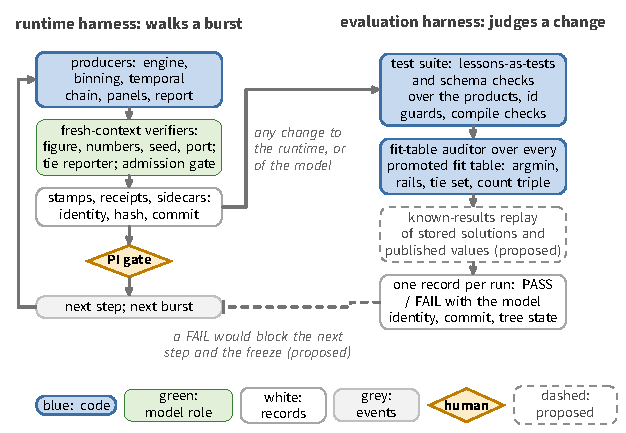
\includegraphics[width=\columnwidth]{figures/fig_F8_eval_harness.pdf}
\caption{Two harnesses. Left, the runtime harness that walks a burst:
producers, fresh-context verifiers, stamps, and the human gate. Right, the
evaluation harness that judges a change to the runtime: the test suite,
the fit-table auditor over every promoted table, and the proposed
known-results replay, run as one command whose record carries the model
identity and the commit (counts at the 2026 September~3 census). Every
change to the runtime harness, and every change of model, is a reason to
run the right-hand side, but that trigger is a discipline rather than a
hook: the pre-commit gate that would enforce it is proposed. The counts are
the census of 2026 September~3, and the promoted tables are those of the
twenty-five bursts promoted so far. The dashed return, a failed battery
blocking the next step and the freeze, is proposed: today the battery
records its verdict and nothing yet consumes it.}
\label{fig:evalharness}
\end{figure}

\subsection{What generalizes}

Gates with stamps, lessons-as-tests, blind-first frozen predictions,
frame alignment before any diff, independence at the primitive, and the
failure taxonomy are domain-agnostic and export as a package; the engine,
the menu, and the lessons' content are the domain deposit that makes the
package worth executing. Both are released. The level at which the package
is designed is the component: the roster of Table~\ref{tab:roster} is the
unit a second group would reproduce, and the science-specific behaviour
harness, the numbers discipline and the blind-first rule, is what a physics
pipeline adds to the generic parts. The skill library, the register, the
role contracts, and the doctrine are text and transfer unchanged across
vendor agent platforms; the enforcement layer, hooks, state derivation,
cascades, is rebuilt per platform. We treat that portability as an
experiment rather than an assumption: the same law executed by a second
vendor's agent on a known burst, compared gate by gate, is the designed
test, and it is pending.

\subsection{Outlook: the discovery plane} \label{sec:creativity}

The production plane described in this paper deliberately excludes
open-ended discovery; a second, sandboxed plane exists for it, governed by
one rule: the agent may invent a new scorecard after seeing the game, but
may not pretend the scorecard was chosen before the game. What would make
that plane generative rather than merely permitted is a hypothesis we are
developing: that creative scientific acts are, predominantly, typed
operations on the knowledge graph of the literature, drawing an edge along
a long or never-co-cited path, negating a named load-bearing assumption of
a published derivation, or constructing a new graph element outright
\citep{boden2004,swanson1986,2013Sci...342..468U,2013arXiv1302.6906F,wiggins2006}.
The reconciliation protocol already extracts, burst by burst, the
assumption-level statements such a graph requires; the discovery plane is
where they would compound. We state it as a direction, not a result.
